% This LaTeX was auto-generated from MATLAB code.
% To make changes, update the MATLAB code and export to LaTeX again.

\documentclass{article}

\usepackage[utf8]{inputenc}
\usepackage[T1]{fontenc}
\usepackage{lmodern}
\usepackage{graphicx}
\usepackage{color}
\usepackage{hyperref}
\usepackage{amsmath}
\usepackage{amsfonts}
\usepackage{epstopdf}
\usepackage[table]{xcolor}
\usepackage{matlab}

\sloppy
\epstopdfsetup{outdir=./}
\graphicspath{ {./BVAR_SA_images/} }

\matlabhastoc

\matlabmultipletitles

\begin{document}

\label{T_90C5FFC4}
\matlabtitle{Bayesian VAR modeling in MATLAB}

\matlabtableofcontents{Table of Contents}
\label{T_8BD09E57}
\matlabtitle{New features in Econometrics - MATLAB}

\label{H_57ACBFC0}
\matlabheading{Interactive workflows for multivariate models}

\begin{par}
\begin{flushleft}
The \href{https://www.mathworks.com/help/econ/econometricmodeler-app.html}{\textbf{Econometric Modeler}} app enables you to test multiple time series for cointegration among the variables by performing the Engle-Granger cointegration test or the Johansen cointegration test.
\end{flushleft}
\end{par}

\begin{par}
\begin{flushleft}
After assessing the cointegrating relationships among the series, you can fit vector autoregression (VAR) models, including optional exogenous variables (VARX) or vector error-correction (VEC) models. As with univariate models, after working in the app, you can export variables to the MATLAB® workspace and generate code or a report summarizing your session. For more details, \href{https://www.mathworks.com/help/econ/econometric-modeler-overview.html}{Econometric Modeler App Overview}.
\end{flushleft}
\end{par}

\label{H_FDE8D0F6}
\matlabheading{Bayesian VAR models}

\begin{par}
\begin{flushleft}
Econometrics Toolbox™ provides Bayesian vector autoregression (VAR) models for analyzing multivariate time series data from a Bayesian point of view. The \href{https://www.mathworks.com/help/releases/R2020a/econ/bayesvarm.html}{\texttt{bayesvarm}} function creates a Bayesian VAR model object that characterizes the joint prior distribution on the coefficients and innovations covariance matrix. The framework enables you to regularize coefficients by using the Minnesota prior \href{https://www.mathworks.com/help/releases/R2020a/econ/bibliography.html#mw_e4462390-8552-40d7-b2b1-3f07501788b7}{[124]}. This table lists supported prior models, ordered by increasing flexibility and complexity.
\end{flushleft}
\end{par}

\begin{par}
\begin{flushleft}
\href{https://www.mathworks.com/help/releases/R2020a/econ/normalbvarm.html}{\texttt{normalbvarm}}
\end{flushleft}
\end{par}

\begin{itemize}
\setlength{\itemsep}{-1ex}
   \item{\begin{flushleft} Normal model \end{flushleft}}
   \item{\begin{flushleft} Normal coefficients; fixed innovations covariance matrix \end{flushleft}}
\end{itemize}

\begin{par}
\begin{flushleft}
\href{https://www.mathworks.com/help/releases/R2020a/econ/conjugatebvarm.html}{\texttt{conjugatebvarm}}
\end{flushleft}
\end{par}

\begin{itemize}
\setlength{\itemsep}{-1ex}
   \item{\begin{flushleft} Conjugate matrix-normal-inverse-Wishart model \end{flushleft}}
   \item{\begin{flushleft} Dependent coefficients and innovations covariance matrix \end{flushleft}}
\end{itemize}

\begin{par}
\begin{flushleft}
\href{https://www.mathworks.com/help/releases/R2020a/econ/semiconjugatebvarm.html}{\texttt{semiconjugatebvarm}}
\end{flushleft}
\end{par}

\begin{itemize}
\setlength{\itemsep}{-1ex}
   \item{\begin{flushleft} Semiconjugate normal-inverse-Wishart model \end{flushleft}}
   \item{\begin{flushleft} Independent coefficients and innovations covariance matrix \end{flushleft}}
\end{itemize}

\begin{par}
\begin{flushleft}
\href{https://www.mathworks.com/help/releases/R2020a/econ/diffusebvarm.html}{\texttt{diffusebvarm}}
\end{flushleft}
\end{par}

\begin{itemize}
\setlength{\itemsep}{-1ex}
   \item{\begin{flushleft} Diffuse model \end{flushleft}}
   \item{\begin{flushleft} Joint prior distribution is inversely proportional to the determinant of the innovations covariance matrix \end{flushleft}}
\end{itemize}

\label{H_F2E6B607}
\matlabheading{Bayesian State Spate Models}

\begin{par}
\begin{flushleft}
A new Bayesian state-space models for analyzing multivariate time series data from a Bayesian point of view. The \href{https://www.mathworks.com/help/econ/bssm.html}{\texttt{bssm}} function creates a Bayesian state-space model (\texttt{bssm} object) that characterizes the joint prior distribution on the state and observation equation parameters, including coefficient, state-disturbance-loading, and observation-innovation matrices.
\end{flushleft}
\end{par}

\begin{par}
\begin{flushleft}
The framework enables you to create a Bayesian state-space model in two ways:
\end{flushleft}
\end{par}

\begin{itemize}
\setlength{\itemsep}{-1ex}
   \item{\begin{flushleft} Convert a standard state-space model (\href{https://www.mathworks.com/help/econ/ssm-class.html}{\texttt{ssm}} object) to a Bayesian state-space model by using the \href{https://www.mathworks.com/help/econ/ssm2bssm.html}{\texttt{ssm2bssm}} function. \end{flushleft}}
   \item{\begin{flushleft} For maximum flexibility, pass the following inputs to \texttt{bssm}: (1) A parameter-to-matrix mapping function that specifies the structure of the state-space model and determines the likelihood computed by the Kalman filter (2) A prior distribution of the parameters, a function representing the log prior or matrix of random draws from the distribution \end{flushleft}}
\end{itemize}

\begin{par}
\begin{flushleft}
After creating a Bayesian state-space model, you can combine the prior model with data to form and analyze the posterior distribution. The data likelihood is formed by assuming that the state disturbances and observation innovations are multivariate Gaussian random variables with a mean of 0. The posterior distribution does not have a closed form; the framework uses Metropolis-Hastings to sample from the posterior. Posterior distribution formation and analysis functions include:
\end{flushleft}
\end{par}

\begin{itemize}
\setlength{\itemsep}{-1ex}
   \item{\begin{flushleft} \href{https://www.mathworks.com/help/econ/bssm.estimate.html}{\texttt{estimate}} – Estimate moments of the posterior distribution given the state-space model structure, data, and initial values for optimization. \end{flushleft}}
   \item{\begin{flushleft} \href{https://www.mathworks.com/help/econ/bssm.simulate.html}{\texttt{simulate}} – Draw random state-space model parameters for custom Monte Carlo estimation. \end{flushleft}}
   \item{\begin{flushleft} \href{https://www.mathworks.com/help/econ/bssm.tune.html}{\texttt{tune}} – Compute proposal distributions for the Metropolis-Hasting sampler to facilitate Monte Carlo simulation. \end{flushleft}}
\end{itemize}


\label{T_503BD93D}
\matlabtitle{BVAR models}

\begin{par}
\begin{flushleft}
Bayesian VAR (BVAR) models have the same mathematical form as any other \textbf{VAR model}, i.e.
\end{flushleft}
\end{par}

\begin{par}
$$y_t =c+\sum_{l=i}^p A_i y_{t-i} +\epsilon_t$$
\end{par}

\begin{par}
\begin{flushleft}
where $y_t$ is a $K\times 1$ vector of endogenous variables in period $t$, $A_i$ is the cofficient matrix corresponding to the $i^{th}$ lag of $y_t$, $c$ is a constant deterministic term and $\epsilon$ is an error term with zero mean and variance-covariance $\Sigma$.
\end{flushleft}
\end{par}

\begin{par}
\begin{flushleft}
The only difference between usual VAR models and BVAR models is the way parameter estimates are obtained and interpreted. VAR models are usually estimated by OLS (ordinary least squares), which is a simple and computationally fast estimator. By contrast, Bayesian estimators are slightly more complicated and more burdensome in terms of algebra and calculation power. The coefficients obtained by so-called \textit{frequentist} estimators like OLS are interpreted based on the concept of the \href{https://en.wikipedia.org/wiki/Sampling_distribution}{\textbf{sampling distribution}}. In Bayesian inference, the coefficients are assumed to have their own distribution. A more detailed treatment of the difference between frequentist and Bayesian inference can be found in Kennedy (2008, ch. 14), which provides a short introduction to the Bayesian approach and a series of references for interested readers. Koop and Korobilis (2010) provide a very good introduction to Bayesian VAR estimators.
\end{flushleft}
\end{par}

\begin{par}
\begin{flushleft}
\textbf{Prior distributrion}
\end{flushleft}
\end{par}

\begin{par}
\begin{flushleft}
$\pi (A)$:  distribution of the parameters of the VAR model based on the observed frequency of a sample.
\end{flushleft}
\end{par}

\begin{par}
\begin{flushleft}
\textbf{Posterior distribution}
\end{flushleft}
\end{par}

\begin{par}
\begin{flushleft}
$\pi (A|y)$: distribution of the parameters of the VAR model based on the observed frequency of the sample
\end{flushleft}
\end{par}

\begin{par}
\begin{flushleft}
\textbf{Bayes theorem}
\end{flushleft}
\end{par}

\begin{par}
$$\pi (A|y)=\frac{\pi (y|A)\pi (y)}{\pi (A)}$$
\end{par}

\begin{par}
\begin{flushleft}
As already mentioned, Bayesian inference can be algebraically demanding. However, Bayesian estimators for linear VAR models can be implemented in a straightforward manner. A standard implementation is a so-called \textbf{Gibbs sampler}, which belongs to the family of Markov-Chain-Monte-Carlo (MCMC) methods. A detailed treatment of this method is beyond the scope of this document, but \href{https://en.wikipedia.org/wiki/Gibbs_sampling}{\textbf{Wikipedia}} might be a good start to become familiar with it. Personally, I like to think of the Gibbs sampler as throwing a bunch of random numbers at a model and see what sticks. The remainer of this text provides the code to set up and estimate a basic BVAR model with MATLAB.
\end{flushleft}
\end{par}


\label{H_F23158B0}
\matlabheading{Monetary Policy in a Trivariate VAR}

\begin{par}
\begin{flushleft}
Let's consider a model for studying monetary policies involving three macroeconomic variables: the inflation rate, the unemployment rate and the interest rate, which are assumed to follow a vector autoregression (VAR) process. We could interpret the unexpected change of the interest rate as the monetary policy shock. This model is studied by Cogley and Sargent (2005), Primiceri (2005) and Koop and Korobilis (2009), among others.
\end{flushleft}
\end{par}

\begin{par}
\begin{flushleft}
Our bash tasks closely follow the empirical illustration of Bayesian VAR in \href{http://personal.strath.ac.uk/gary.koop/kk3.pdf}{Koop and Korobilis (2010)}.
\end{flushleft}
\end{par}

\begin{par}
\begin{flushleft}
To illustrate Bayesian VAR methods using some of the priors and methods described above, we use a quarterly US data set on the inflation rate $\Delta \pi_t$ (the annual percentage change in a chain-weighted GDP price index), the unemployment rate $u_t$ (seasonally adjusted civilian unemployment rate, all workers over age 16) and the interest rate $r_t$ (yield on the three month Treasury bill rate). Thus $y_t =(\Delta \pi_t ,u_t ,r_t )^{\prime }$. The sample runs from 1953Q1 to 2006Q3. These three variables are commonly used in New Keynesian VARs.
\end{flushleft}
\end{par}

\begin{matlabcode}
clear;

c = fred('https://research.stlouisfed.org/fred2');
c.DatetimeType = 'datetime';
c.DataReturnFormat = 'timetable';

startdate = datetime(1953,1,1);
enddate = datetime(2006, 7, 1);

inflation    = c.fetch('B191RO1Q156NBEA', startdate , enddate );
inflation = inflation.Data{1};
unemployment = c.fetch('UNRATE', startdate , enddate ); unemployment = unemployment.Data{1};
unemployment = retime(unemployment,"regular","fillwithmissing",...
    "TimeStep",calquarters(1));
interest     = c.fetch('TB3MS', startdate , enddate ); interest = interest.Data{1};
interest = retime(interest,"regular","fillwithmissing","TimeStep",calquarters(1));

% Synchronize timetables
Table = synchronize(inflation,interest,unemployment,"union",...
    "fillwithmissing");
Table.Properties.VariableNames = {'inflation', 'unemployment', 'interest'};

Y = Table{:,:};
figure;
stackedplot(Table)
\end{matlabcode}
\begin{center}
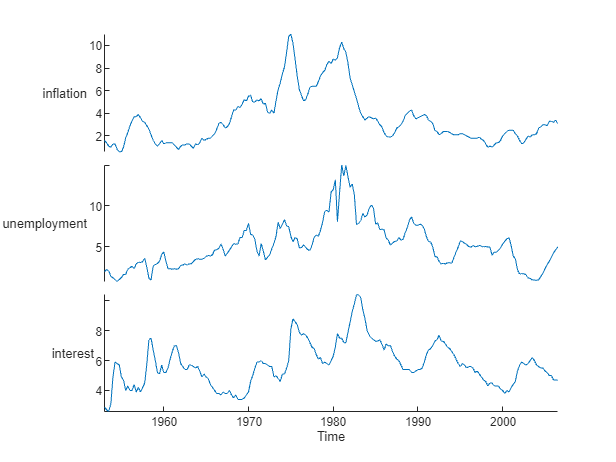
\includegraphics[width=\maxwidth{56.096337180130455em}]{figure_0.png}
\end{center}


\label{H_CF3CD0CF}
\begin{par}
\begin{flushleft}
To illustrate Bayesian VAR analysis using this data, we work with an unrestricted VAR with an intercept and four lags of all variables included in every equation and consider the following priors:
\end{flushleft}
\end{par}

\begin{itemize}
\setlength{\itemsep}{-1ex}
   \item{\begin{flushleft} \href{https://www.mathworks.com/help/econ/diffusebvarm.html#mw_d9bd0d93-e75f-449d-b599-7392399317c2}{\textbf{Noninformative}}\textbf{:} The diffuse model is the limiting case of the natural conjugate when $M\to 0,V^{-1} \to 0,\Omega \to 0,$ and $\nu \to -k$ \end{flushleft}}
   \item{\begin{flushleft} \href{https://www.mathworks.com/help/econ/conjugatebvarm.html#mw_984677e2-0799-4589-a86b-b2e98366d114}{\textbf{Natural conjugate}}\textbf{: }The \textit{dependent, matrix-normal-inverse-Wishart conjugate model} is an \textit{m}-D Bayesian VAR(\textit{p}) model in which the conditional prior distribution of $\Lambda |\Sigma$ is matrix normal with mean matrix $M$ and scale matrices $\Sigma$ and $V$. The prior distribution of $\Sigma$ is inverse Wishart with scale matrix $\Omega$ and degrees of freedom $\nu$\textit{.} \end{flushleft}}
   \item{\begin{flushleft} \href{https://www.mathworks.com/help/econ/normalbvarm.html#mw_79c1a524-2701-4c6a-ab97-e2a5ac17fca8}{\textbf{Minnesota}}\textbf{:} Fixed Innovations Matrix $\Sigma$, while the coefficient vector follows a normal distribution. \end{flushleft}}
   \item{\begin{flushleft} \href{https://www.mathworks.com/help/econ/semiconjugatebvarm.html#mw_bccf0fa5-38e1-43f5-8554-6ca69110db4c}{\textbf{Independent Normal-Wishart}}\textbf{:} The \textit{independent, normal-inverse-Wishart semiconjugate model} is an \textit{m}-D Bayesian VAR model in which the conditional prior distribution of $\lambda |\Sigma$ is multivariate normal with mean vector \textit{μ} and covariance matrix \textit{V}. The prior distribution of Σ is inverse Wishart with scale matrix Ω and degrees of freedom \textit{ν}. \end{flushleft}}
\end{itemize}

\begin{par}
\begin{flushleft}
For the first three priors, analytical posterior and predictive results are available. For last one, posterior and predictive simulation is required.
\end{flushleft}
\end{par}

\begin{matlabcode}
numSeries = 3;
numLags = 4;
priorType = "Minnesota";
seriesNames = ["pi", "ut", "rt"];

MdlF = varm(numSeries,numLags);
EstMdlF = estimate(MdlF,Y);
\end{matlabcode}
\begin{matlaboutput}
Unrecognized function or variable 'Y'.
\end{matlaboutput}
\begin{matlabcode}

[Mdl, EstMdl] = estimateBayesVARM(numSeries, numLags, priorType, seriesNames, Y, EstMdlF);
disp("The Prior model is of type: " + class(Mdl))
disp("The Posterior model is of type: " + class(EstMdl))
disp("The following is the model summary")
summarize(EstMdl)
\end{matlabcode}


\label{H_5ADC58EB}
\matlabheadingtwo{Impulse response functions}

\begin{par}
\begin{flushleft}
(Deeper dive \href{..\Internal\IRF.mlx}{here})
\end{flushleft}
\end{par}

\begin{par}
\begin{flushleft}
In empirical studies, the VAR coefficients\textit{ per se} are rarely of direct interest since it hard to interpret them. Instead, the main interest lies in some nonlinear transformations of those coefficients such as the impulse response analysis. Currently, we have obtained the reduced-form VAR, which needs identification restrictions to recover the structural-form VAR. In this model, the identification conditions can be a specific variable order: inflation, unemployment and interest rate. That is, the interest rate shock does not have a contemporaneous effect on the other two variables, which reflects the time lag of the responses to the monetary policy shock.
\end{flushleft}
\end{par}

\begin{par}
\begin{flushleft}
Now we extract the posterior mean of the estimated model and construct VARM for the impulse response analysis.
\end{flushleft}
\end{par}

\begin{matlabcode}
mdl = varm('Constant',EstMdl.Constant,'AR',EstMdl.AR, 'Covariance',EstMdl.Covariance);
Response = irf(mdl,'NumObs',24);
\end{matlabcode}


\begin{par}
\begin{flushleft}
With the structural shocks identified by the lower triangular constraints, we could interpret the unexpected change of interest rate as a monetary policy shock. As the interest rate rises, a contractionary monetary policy will reduce the inflation rate, lower the outputs and increase the unemployment rate, if the money is not a veil on the real economy.
\end{flushleft}
\end{par}

\begin{par}
\begin{flushleft}
Note: we will plot the responses to one unit of shock, instead of one standard deviation of shock.
\end{flushleft}
\end{par}

\begin{matlabcode}
t = tiledlayout(3, 3);
names = ["pi", "u", "r"];
s2 = diag(EstMdlF.Covariance);
for i = 1 : 3
    for j = 1 : 3

        ax = nexttile(t);
        plot(ax, Response(:,i,j) ./ sqrt(s2(1)));
        title(names(i) + " -> " + names(j))

    end
end
\end{matlabcode}
\begin{center}
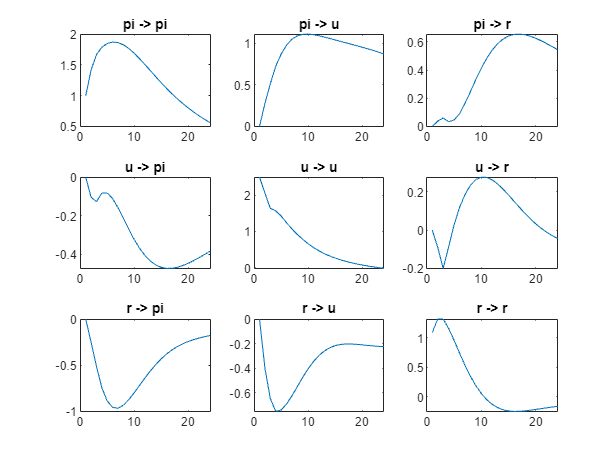
\includegraphics[width=\maxwidth{56.096337180130455em}]{figure_1.png}
\end{center}


\label{H_BC2B00B2}
\matlabheadingthree{Computing IRF intervals by Monte Carlo}

\begin{par}
\begin{flushleft}
First, we can simulate many posterior draws of VAR coefficients and the covariance matrix. For each draw, we construct a VARM model and compute the impulse response functions. Repeat the process for all draws, we obtain a collection of impulse response functions. After sorting them we can compute the quantiles (say 5\% and 95\%), which constitute a band that characterizes the uncertainties on the impulse response functions. Example code:
\end{flushleft}
\end{par}

\begin{matlabcode}
numDraws = 500;
if isa(EstMdl, 'empiricalbvarm')
    draws = randsample(10000,numDraws);
    Coeff = EstMdl.CoeffDraws(:, draws);
    Sigma = EstMdl.SigmaDraws(:, :, draws);
else
    [Coeff,Sigma] = simulate(EstMdl,'NumDraws',numDraws);
end
Response4D = zeros(24,3,3,numDraws);
for m = 1:numDraws
    A = reshape(Coeff(:,m),13,3)';
    mdl = varm('Constant',A(:,13),'AR',{A(:,1:3),A(:,4:6),A(:,7:9),A(:,10:12)},'Covariance',Sigma(:,:,m));
    Response4D(:,:,:,m) = irf(mdl,'NumObs',24);
end
Response05 = quantile(Response4D,0.05,4);
Response95 = quantile(Response4D,0.95,4);
t = tiledlayout(3, 3);
names = ["pi", "u", "r"];
for i = 1 : 3
    for j = 1 : 3

        ax = nexttile();
        plot(ax, Response(:,i,j) ./ sqrt(s2(1)));
        title(names(i) + " -> " + names(j))
        hold on
        plot(ax, Response05(:,i,j) ./ sqrt(s2(1)), 'r--')
        plot(ax, Response95(:,i,j) ./ sqrt(s2(1)), 'r--')
        hold off

    end
end
\end{matlabcode}
\begin{center}
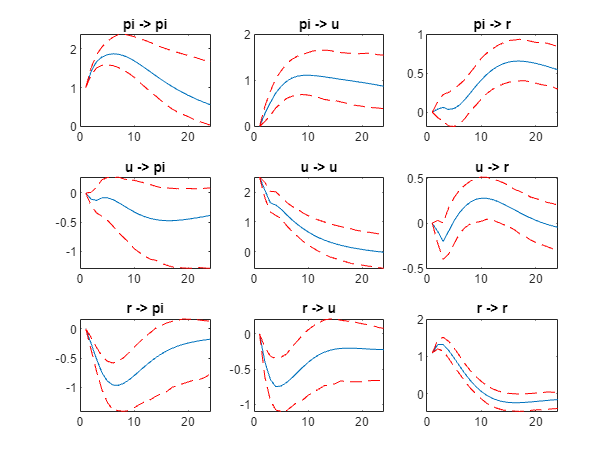
\includegraphics[width=\maxwidth{56.096337180130455em}]{figure_2.png}
\end{center}


\label{T_D0EC6A5E}
\matlabtitle{Other resources}

\begin{par}
\begin{flushleft}
\href{https://github.com/european-central-bank/BEAR-toolbox}{BEAR toolbox}
\end{flushleft}
\end{par}

\begin{par}
\begin{flushleft}
The Bayesian Estimation, Analysis and Regression toolbox (BEAR) is a comprehensive (Bayesian Panel) VAR toolbox for forecasting and policy analysis.
\end{flushleft}
\end{par}

\begin{par}
\begin{flushleft}
BEAR is a MATLAB based toolbox which is easy for non-technical users to understand, augment and adapt. In particular, BEAR includes a user-friendly graphical interface which allows the tool to be used by country desk economists.
\end{flushleft}
\end{par}

\begin{par}
\begin{flushleft}
Furthermore, BEAR is well documented, both within the code as well as including a detailed theoretical and user’s guide. BEAR includes state-of-the art applications such as FAVARs, stochastic volatility, time-varying parameters, mixed-frequency, sign and magnitude restrictions, conditional forecasts, Bayesian forecast evaluation measures, Bayesian Panel VAR using different prior distributions (for example hierarchical priors).
\end{flushleft}
\end{par}

\begin{par}
\begin{flushleft}
BEAR is specifically developed for transparently supplying a tool for state-of-the-art research and is planned to be further developed to always be at the frontier of economic research.
\end{flushleft}
\end{par}

\begin{par}
\begin{flushleft}
Use of BEAR implies acceptance of the End User \href{https://github.com/european-central-bank/BEAR-toolbox#License}{Licence Agreement (EULA)} for the Use of the Software “the Bayesian Estimation, Analysis and Regression (BEAR) toolbox”.
\end{flushleft}
\end{par}

\begin{verbatim}
BEARapp; % Run this command if you have the BEAR toolbox installed.
\end{verbatim}

\begin{par}
\begin{flushleft}
\href{https://www.dynare.org/}{Dynare}
\end{flushleft}
\end{par}

\begin{par}
\begin{flushleft}
Dynare is a software platform for handling a wide class of economic models, in particular dynamic stochastic general equilibrium (DSGE) and overlapping generations (OLG) models. The models solved by Dynare include those relying on the rational expectations hypothesis, wherein agents form their expectations about the future in a way consistent with the model. But Dynare is also able to handle models where expectations are formed differently: on one extreme, models where agents perfectly anticipate the future; on the other extreme, models where agents have limited rationality or imperfect knowledge of the state of the economy and, hence, form their expectations through a learning process. In terms of types of agents, models solved by Dynare can incorporate consumers, productive firms, governments, monetary authorities, investors and financial intermediaries. Some degree of heterogeneity can be achieved by including several distinct classes of agents in each of the aforementioned agent categories.
\end{flushleft}
\end{par}

\begin{par}
\begin{flushleft}
Dynare offers a user-friendly and intuitive way of describing these models. It is able to perform simulations of the model given a calibration of the model parameters and is also able to estimate these parameters given a dataset. In practice, the user will write a text file containing the list of model variables, the dynamic equations linking these variables together, the computing tasks to be performed and the desired graphical or numerical outputs.
\end{flushleft}
\end{par}

\begin{par}
\begin{flushleft}
A large panel of applied mathematics and computer science techniques are internally employed by Dynare: multivariate nonlinear solving and optimization, matrix factorizations, local functional approximation, Kalman filters and smoothers, MCMC techniques for Bayesian estimation, graph algorithms, optimal control, etc. References to the literature can be found \href{https://www.dynare.org/bibliography}{here}.
\end{flushleft}
\end{par}

\begin{verbatim}
launchDynare % Run this command if you have the Dynare editor installed.
\end{verbatim}
\begin{par}
\begin{flushleft}
\textbf{SAMNet is a repository of models for modelling and forecasting the economy}
\end{flushleft}
\end{par}

\begin{matlabcode}
web('https://samnet.org.za/model-databases/','browser')
\end{matlabcode}


\begin{matlabcode}
edit SamNet.mod
\end{matlabcode}


\begin{matlabcode}
dynare SamNet.mod
\end{matlabcode}
\begin{matlaboutput}
Starting Dynare (version 5.3).
Calling Dynare with arguments: none
Starting preprocessing of the model file ...
Found 19 equation(s).
Evaluating expressions...done
Computing static model derivatives (order 1).
Computing dynamic model derivatives (order 1).
Processing outputs ...
done
Preprocessing completed.


STEADY-STATE RESULTS:

C      		 0.31994
C_h    		 0.2941
C_e    		 0.0216553
C_b    		 0.00418431
H_h    		 0.748768
H_e    		 0.251232
N      		 0.32865
W      		 0.876146
q      		 4.36421
D      		 0.677659
L_e    		 0.757161
R_d    		 1.00908
R_l    		 1.01365
Sprd   		 0.00457273
Y      		 0.31994
kappa  		 0.105
A      		 1
Z      		 1
vareps 		 0

EIGENVALUES:
         Modulus             Real        Imaginary

       1.903e-09       -1.903e-09                0
       1.903e-09        1.903e-09                0
       1.559e-08        1.559e-08                0
       1.559e-08       -1.559e-08                0
          0.5877           0.5877                0
          0.6759           0.6759                0
          0.6979           0.6979                0
             0.8              0.8                0
             0.8              0.8                0
             0.9              0.9                0
           0.931            0.931                0
           1.011            1.011                0
           1.049            1.049                0
           1.062            1.062                0
           1.652           -1.652                0
        9.19e+17        -9.19e+17                0
             Inf              Inf                0


There are 6 eigenvalue(s) larger than 1 in modulus 
for 6 forward-looking variable(s)

The rank condition is verified.


MODEL SUMMARY

  Number of variables:         19
  Number of stochastic shocks: 3
  Number of state variables:   11
  Number of jumpers:           6
  Number of static variables:  5


MATRIX OF COVARIANCE OF EXOGENOUS SHOCKS
Variables          ups_a       ups_z  ups_vareps
ups_a           0.000000    0.000000    0.000000
ups_z           0.000000    0.000100    0.000000
ups_vareps      0.000000    0.000000    0.000000

POLICY AND TRANSITION FUNCTIONS
                                   C             C_h             C_e             C_b             H_h             H_e               N               W               q               D             L_e             R_d             R_l            Sprd               Y           kappa               A               Z          vareps
Constant                    0.319940        0.294100        0.021655        0.004184        0.748768        0.251232        0.328650        0.876146        4.364208        0.677659        0.757161        1.009082        1.013654        0.004573        0.319940        0.105000        1.000000        1.000000               0
H_h(-1)                     0.796128        0.644542        0.104758        0.046828       -2.647356        2.647356       -4.072471        1.085676       33.833080       12.062007       14.843113       -6.974537        3.734918       10.709455       -3.568080        1.614689               0               0               0
H_e(-1)                     0.933362        0.677875        0.183908        0.071578       -5.303482        5.303482       -4.061188        1.431408       37.439522       19.379862       23.508757       -6.180095        5.547661       11.727755       -3.430846        2.193028               0               0               0
D(-1)                      -0.018000        0.003252       -0.016196       -0.005055        0.564827       -0.564827       -0.020545        0.005477       -0.255536       -1.475391       -1.748552       -0.300361        0.965271        1.265633       -0.018000       -0.118287               0               0               0
L_e(-1)                    -0.001428        0.000258       -0.000902       -0.000784       -0.002205        0.002205       -0.001630        0.000434        0.015679        0.008078        0.009799       -0.000222       -1.337519       -1.337297       -0.001428        0.000914               0               0               0
R_d(-1)                    -0.012088        0.002184       -0.010877       -0.003395        0.379315       -0.379315       -0.013797        0.003678       -0.171608       -0.990814       -1.174258       -0.201711        0.648238        0.849949       -0.012088       -0.079437               0               0               0
A(-1)                       0.000549       -0.000099        0.000522        0.000126       -0.009798        0.009798        0.000627       -0.000167        0.145073        0.043355        0.051379        0.005257        0.010764        0.005507        0.000549        0.003472        0.800000               0               0
Z(-1)                       0.119672        0.095202        0.018758        0.005712       -0.413517        0.413517       -0.155544        0.742383        5.029514        1.817178        2.139240       -0.129168        0.432899        0.562067        0.119672        0.128693               0        0.800000               0
vareps(-1)                 -0.005939        0.001073       -0.013588        0.006576        0.465540       -0.465540       -0.006779        0.001807       -0.057905       -2.038130       -1.350021       -0.258494        0.917487        1.175982       -0.005939       -0.092633               0               0        0.900000
C_h(-1)                     0.572596        0.596566       -0.017151       -0.006818        0.373666       -0.373666        0.653539       -0.174226       -5.363836       -1.711986       -2.116472        0.298899       -0.543220       -0.842119        0.572596       -0.240711               0               0               0
C_e(-1)                     0.535169       -0.096674        0.642606       -0.010763        0.717473       -0.717473        0.610822       -0.162838       -5.856670       -2.552874       -3.109040        0.147536       -0.748756       -0.896292        0.535169       -0.303392               0               0               0
C_b(-1)                     0.538170       -0.097216       -0.029119        0.664505        0.962821       -0.962821        0.614247       -0.163751       -5.933048       -3.620381       -4.376553        0.005761       -0.121067       -0.126828        0.538170       -0.391771               0               0               0
ups_a                       0.000686       -0.000124        0.000653        0.000157       -0.012248        0.012248        0.000783       -0.000209        0.181341        0.054194        0.064224        0.006572        0.013455        0.006883        0.000686        0.004341        1.000000               0               0
ups_z                       0.149590        0.119002        0.023447        0.007141       -0.516896        0.516896       -0.194431        0.927979        6.286893        2.271473        2.674050       -0.161460        0.541123        0.702584        0.149590        0.160866               0        1.000000               0
ups_vareps                 -0.006599        0.001192       -0.015098        0.007307        0.517266       -0.517266       -0.007532        0.002008       -0.064339       -2.264589       -1.500023       -0.287216        1.019431        1.306646       -0.006599       -0.102926               0               0        1.000000


THEORETICAL MOMENTS
VARIABLE         MEAN  STD. DEV.   VARIANCE
C              0.3199     0.0069     0.0000
C_h            0.2941     0.0052     0.0000
C_e            0.0217     0.0014     0.0000
C_b            0.0042     0.0003     0.0000
H_h            0.7488     0.0158     0.0003
H_e            0.2512     0.0158     0.0003
N              0.3287     0.0028     0.0000
W              0.8761     0.0188     0.0004
q              4.3642     0.1088     0.0118
D              0.6777     0.0558     0.0031
L_e            0.7572     0.0652     0.0043
R_d            1.0091     0.0048     0.0000
R_l            1.0137     0.0078     0.0001
Sprd           0.0046     0.0075     0.0001
Y              0.3199     0.0069     0.0000
kappa          0.1050     0.0034     0.0000
A              1.0000     0.0000     0.0000
Z              1.0000     0.0167     0.0003
vareps         0.0000     0.0000     0.0000



VARIANCE DECOMPOSITION (in percent)
               ups_a       ups_z  ups_vareps
C               0.00      100.00        0.00
C_h             0.00      100.00        0.00
C_e             0.00      100.00        0.00
C_b             0.00      100.00        0.00
H_h             0.00      100.00        0.00
H_e             0.00      100.00        0.00
N               0.00      100.00        0.00
W               0.00      100.00        0.00
q               0.00      100.00        0.00
D               0.00      100.00        0.00
L_e             0.00      100.00        0.00
R_d             0.00      100.00        0.00
R_l             0.00      100.00        0.00
Sprd            0.00      100.00        0.00
Y               0.00      100.00        0.00
kappa           0.00      100.00        0.00
A             100.00        0.00        0.00
Z               0.00      100.00        0.00
vareps          0.00        0.00      100.00



MATRIX OF CORRELATIONS
Variables          C      C_h      C_e      C_b      H_h      H_e        N        W        q        D      L_e      R_d      R_l     Sprd        Y    kappa        Z
C             1.0000   0.9958   0.9609   0.9671  -0.9692   0.9692   0.2061   0.9212   0.8605   0.9662   0.9651  -0.8240  -0.4815   0.0282   1.0000   0.9390   0.8410
C_h           0.9958   1.0000   0.9315   0.9402  -0.9482   0.9482   0.1601   0.9353   0.8785   0.9561   0.9550  -0.8552  -0.4898   0.0397   0.9958   0.9270   0.8670
C_e           0.9609   0.9315   1.0000   0.9975  -0.9803   0.9803   0.3442   0.8271   0.7564   0.9435   0.9427  -0.6831  -0.4384  -0.0176   0.9609   0.9224   0.7139
C_b           0.9671   0.9402   0.9975   1.0000  -0.9914   0.9914   0.2783   0.8596   0.7969   0.9634   0.9628  -0.7206  -0.4080   0.0384   0.9671   0.9468   0.7550
H_h          -0.9692  -0.9482  -0.9803  -0.9914   1.0000  -1.0000  -0.1533  -0.9113  -0.8639  -0.9891  -0.9889   0.7756   0.3300  -0.1554  -0.9692  -0.9804  -0.8267
H_e           0.9692   0.9482   0.9803   0.9914  -1.0000   1.0000   0.1533   0.9113   0.8639   0.9891   0.9889  -0.7756  -0.3300   0.1554   0.9692   0.9804   0.8267
N             0.2061   0.1601   0.3442   0.2783  -0.1533   0.1533   1.0000  -0.1908  -0.3205   0.0206   0.0177   0.2899  -0.5902  -0.8041   0.2061  -0.0446  -0.3492
W             0.9212   0.9353   0.8271   0.8596  -0.9113   0.9113  -0.1908   1.0000   0.9907   0.9610   0.9612  -0.9419  -0.2484   0.3480   0.9212   0.9597   0.9825
q             0.8605   0.8785   0.7564   0.7969  -0.8639   0.8639  -0.3205   0.9907   1.0000   0.9286   0.9291  -0.9436  -0.1478   0.4543   0.8605   0.9376   0.9941
D             0.9662   0.9561   0.9435   0.9634  -0.9891   0.9891   0.0206   0.9610   0.9286   1.0000   1.0000  -0.8479  -0.2890   0.2449   0.9662   0.9959   0.8996
L_e           0.9651   0.9550   0.9427   0.9628  -0.9889   0.9889   0.0177   0.9612   0.9291   1.0000   1.0000  -0.8478  -0.2858   0.2482   0.9651   0.9963   0.9001
R_d          -0.8240  -0.8552  -0.6831  -0.7206   0.7756  -0.7756   0.2899  -0.9419  -0.9436  -0.8479  -0.8478   1.0000   0.3776  -0.2504  -0.8240  -0.8427  -0.9376
R_l          -0.4815  -0.4898  -0.4384  -0.4080   0.3300  -0.3300  -0.5902  -0.2484  -0.1478  -0.2890  -0.2858   0.3776   1.0000   0.8019  -0.4815  -0.2170  -0.1299
Sprd          0.0282   0.0397  -0.0176   0.0384  -0.1554   0.1554  -0.8041   0.3480   0.4543   0.2449   0.2482  -0.2504   0.8019   1.0000   0.0282   0.3168   0.4691
Y             1.0000   0.9958   0.9609   0.9671  -0.9692   0.9692   0.2061   0.9212   0.8605   0.9662   0.9651  -0.8240  -0.4815   0.0282   1.0000   0.9390   0.8410
kappa         0.9390   0.9270   0.9224   0.9468  -0.9804   0.9804  -0.0446   0.9597   0.9376   0.9959   0.9963  -0.8427  -0.2170   0.3168   0.9390   1.0000   0.9058
Z             0.8410   0.8670   0.7139   0.7550  -0.8267   0.8267  -0.3492   0.9825   0.9941   0.8996   0.9001  -0.9376  -0.1299   0.4691   0.8410   0.9058   1.0000



COEFFICIENTS OF AUTOCORRELATION
Order           1        2        3        4        5
C          0.9648   0.8920   0.8059   0.7191   0.6378
C_h        0.9595   0.8746   0.7748   0.6755   0.5839
C_e        0.9812   0.9428   0.8947   0.8423   0.7890
C_b        0.9734   0.9298   0.8798   0.8280   0.7767
H_h        0.9450   0.8899   0.8359   0.7836   0.7336
H_e        0.9450   0.8899   0.8359   0.7836   0.7336
N          0.6381   0.3305   0.1606   0.0694   0.0226
W          0.8679   0.7228   0.6075   0.5148   0.4396
q          0.8139   0.6336   0.5074   0.4163   0.3486
D          0.9130   0.8282   0.7567   0.6947   0.6399
L_e        0.9118   0.8265   0.7551   0.6935   0.6392
R_d        0.8380   0.5816   0.4153   0.3050   0.2299
R_l        0.2597  -0.0192   0.0076   0.0213   0.0276
Sprd       0.1834  -0.1749  -0.1107  -0.0723  -0.0491
Y          0.9648   0.8920   0.8059   0.7191   0.6378
kappa      0.8825   0.7862   0.7168   0.6630   0.6183
Z          0.8000   0.6400   0.5120   0.4096   0.3277
\end{matlaboutput}
\begin{center}
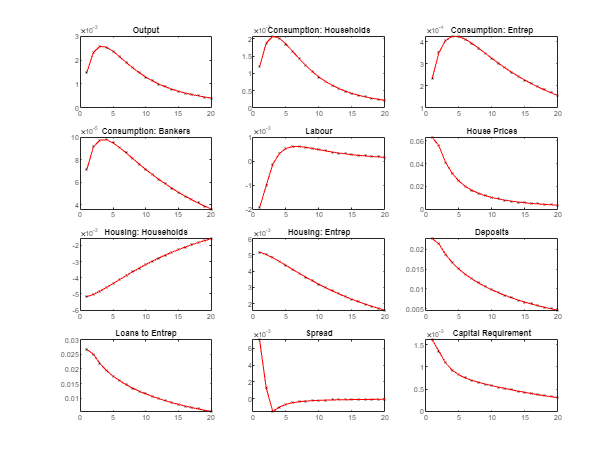
\includegraphics[width=\maxwidth{56.096337180130455em}]{figure_3.png}
\end{center}
\begin{matlaboutput}
Total computing time : 0h00m05s
\end{matlaboutput}


\begin{par}
\begin{flushleft}
\href{https://iris.igpmn.org/}{IRIS toolbox}
\end{flushleft}
\end{par}

\begin{par}
\begin{flushleft}
IRIS is a free, open-source toolbox for macroeconomic modeling and forecasting in Matlab®, originally developed by the IRIS Solutions Team and currently maintained and supported by the Global Projection Model Network.
\end{flushleft}
\end{par}

\begin{par}
\begin{flushleft}
In a user-friendly command-oriented environment, IRIS integrates core modeling functions (including a flexible model file language with a powerful preparser, a variety of tools for simulation, estimation, forecasting and model diagnostics, practical techniques for judgmental adjustments, and more) with supporting infrastructure (such as data management, time series analysis, and reporting).
\end{flushleft}
\end{par}


\label{T_98AC8677}
\matlabtitle{References}

\begin{par}
\begin{flushleft}
[1] Cogley, T. and Sargent, T. (2005). \textbf{Drifts and volatilities: Monetary policies and outcomes in the post WWII} U.S, Review of Economic Dynamics, 8, 262-302.
\end{flushleft}
\end{par}

\begin{par}
\begin{flushleft}
[2] Primiceri. G., (2005). \textbf{Time varying structural vector autoregressions and monetary policy}, Review of Economic Studies, 72, 821-852.
\end{flushleft}
\end{par}

\begin{par}
\begin{flushleft}
[3] Koop, G. and Korobilis, D. (2009). \textbf{Bayesian Multivariate Time Series Methods for Empirical Macroeconomics}, Working Paper series 47-09, Rimini Centre for Economic Analysis.
\end{flushleft}
\end{par}

\end{document}
